\chapter{Introduction}\label{chapter:intro}

  \section{Membranes for Selective Aqueous Separations}
  
  Pressure drive membrane processes have become an increasingly useful tool for
  performing aqueous separations.
  \begin{itemize}
    \item Untreated water can be a very complex solution with particles ranging
    in size from microns down to nanometers
    \item Sediment, bacteria, algae, proteins, small organic molecules, and ions
    are all typical components of aqueous streams.
%    \item Their original intention was for desalination applications but they 
%    have since expanded their reach to a more diverse set of chemical separation
%    problems. 
  \end{itemize}
  
  % BJC: This should probably go up top
  % TFC membranes review -- "Composite reverse osmosis and nanofiltration membranes"
  Membrane design is completely dependent on the target particle separation. 
  \begin{itemize}
    \item We have summarized the uses of different classes of membrane separation 
    technologies in Figure~\ref{fig:size_regimes}
    \item They can be classified based on the size of the particle they reject.
    \item Microfiltration membranes contain 0.1-1.0 $\mu$m pores. (separate bacteria, pigment removal)
    \item Ultrafiltration (sugars, proteins, colloidal materials) pore size about 0.05 $\mu$m
    \item Nanofiltration have pores on the order of 1 nm in size
    \item Reverse osmosis membranes are dense amorphous polymers with no explicit pores
    \item These technologies are often used in series
  \end{itemize}
  
  \begin{figure}
  \centering
  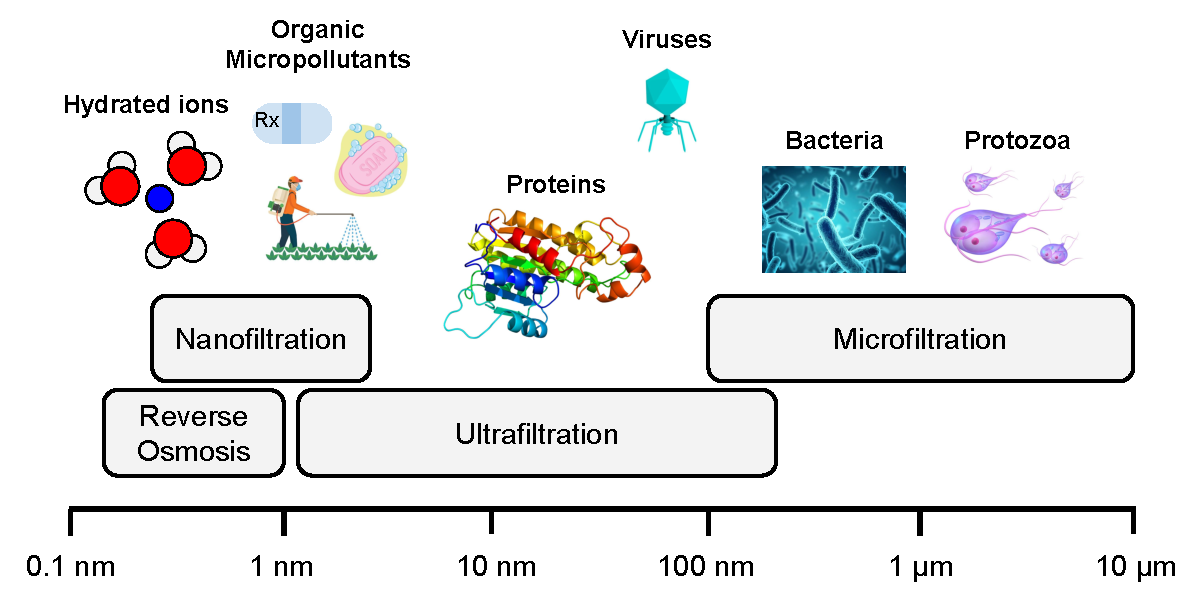
\includegraphics[width=\textwidth]{figs/membrane_separation_size_regimes.pdf}
  \caption{}\label{fig:size_regimes}
  \end{figure}
  
  \subsection{How Small Molecule Membrane Separations Work}
  
  %\wijmans_solution-diffusion_1995
  Membrane permeation is the result of a chemical potential gradient $\frac{d\mu_i}{dx}$.
  \begin{itemize}
	  \item The flux of component $i$ is proportional to this gradient:
	  \begin{equation}
	    J_i = -L_i \frac{d\mu_i}{dx}
	  \end{equation}
	  where $L_i$ is a coefficient of proportionality.
	  \item Chemical potential gradients can be induced by concentration, pressure, 
	  temperature and electromotive force.
  \end{itemize}
  
  % This follows the discussion of werber_material_2016
  For pressure driven membrane processes, water flux through both porous and 
  amorphous membranes can be described by
  \begin{equation}
  J_w = A(\Delta P - \Delta \pi_m)
  \end{equation}
  where $J_w$ is volumetric water flux, $A$ is the water permeability coefficient,
  $\Delta P$ is the applied hydraulic pressure and $\Delta \pi_m$ is the 
  trans-membrane osmotic pressure difference. The water permeability coefficient
  is dependent on how one models flow through the membrane.
  
  In porous membrane architectures, water flux is modeled as laminar flow through 
  cylindrical pores.
  \begin{itemize}
    \item The derivation follows Hagen-Poiseuille flow with inclusion of morphological
    characteristics:
    \begin{equation}
    A = \frac{\varepsilon r_p^2}{8\mu\delta_m}
    \end{equation}
    where $\varepsilon$ is the surface porosity, $r_p$ the pore radius, $\delta_m$ the
    membrane thickness, and $\mu$ the solution viscosity.
    \item Separation is considered in terms of rejection. Solutes with radii smaller
    than the pore will be rejected. A distribution of pore sizes prevents perfect
    rejection.
  \end{itemize}
  
  In amorphous membranes, water flux is modeled using the solution-diffusion 
  model.
  \begin{itemize}
    \item It is hypothesized that water and solute molecules partition into the
    membrane and diffuse across the polymer matrix due to a chemical potential
    gradient and then desorb into the permeate.
    \item The solubility and diffusivity can be described  in terms of the 
    diffusive water and solute permeabilities ($P_w$ and $P_s$) respectively
    \item \begin{equation}
    A = \frac{P_wV_w}{\delta_mR_gT}
    \end{equation}
    where $V_w$ is molar volume of water, $R_g$ is the gas constant and $T$ is
    absolute temperature.
    \item Solute flux is modeled as:
    \begin{equation}
    J_s = \frac{P_s}{\delta_m}\Delta c_m
    \end{equation}
  \end{itemize}
  
  These equations provide a somewhat limited perspective on the molecular details
  of transport. 
  
  
  \subsection{Membrane Separation Applications}
  
  Selective separations are useful for a wide range of applications.  
  
  % Put this with the desalination section below maybe
  % morton_environmental_1996,bhojwani_technology_2019
  \textit{Desalination}:
  Creating potable water from seawater or brackish water is of paramount importance
  in water-scarce areas. 
  \begin{itemize}
  	\item Compared with thermal distillation techniques, reverse osmosis has been 
  	shown to be more environmently friendly and economical due to its lower energy
  	requirements.
  	\item Thermal techniques are still preferred where excess waste heat or cheap 
  	thermal energy is available, such as cogeneration plants.
  	\item RO has smaller footprint?
  \end{itemize}

  \textit{Organic Micropollutants}:
  Municipal and industrial wastewaters are contaminated by harmful
  micropollutants, which have adverse effects on human health even at low 
  concentrations\cite{schwarzenbach_challenge_2006}
  \begin{itemize}
    \item Micropollutants include pharmaceutical and personal care products, 
    hormones, pesticides and industrial chemicals which find their way into
    our drinking water supply
    \item Is there any infrastructure built to combat this?
  \end{itemize}
  
  \textit{Recovery of Valuable Dissolved Species}: We can use highly selective
  membranes in order to recover potentially valueable dissolved species from 
  complex waste streams. 
  
  Municipal waste-waters are rich in carbon, nitrogen and phosphorus-containing 
  compounds. 
  \begin{itemize}  
    \item The recovery of such products, which can be achieved using a 
    selective membrane, has numerous potential uses.\cite{sales_resource_2015}
    \item For example, nitrogen and phosphorus recovery can help sustain fertilizer 
    production which will help meet global food demand as population continues
    to increase.\cite{xie_membrane-based_2016}
  \end{itemize}

  Industrial waste-waters are often quite complex with up to six times more 
  total dissolved solids than seawater\cite{werber_materials_2016}. 
  \begin{itemize}
    \item For example, flowback water, produced during hydraulic fracturing of
    shale formations consists of relatively high concentrations of salts, metals,
    and soluble organic compounds. 
    \item The majority of this water is disposed through deep well injection, 
    however there is a growing public concern about its management which has 
    prompted the use of separation technologies such as RO and NF in order to 
    reduce the volume of contaminated water~\cite{gregory_water_2011}.
    \item Some of the dissolved organic compounds in flowback water, such as acetate, 
    are potentially valuable and can be recovered with highly selective membranes
    \cite{dischinger_application_2017}.
  \end{itemize}
  
  \textit{Breathable barriers}:
  Finally, there is a great deal of military interest in creating breathable 
  barriers which selectively allow the passage of water in both directions but
  blocks out harmful contaminants.
  \begin{itemize}
    \item Need to allow sweating
    \item Can even put catalytic groups in the pores to break down contaminants
  \end{itemize}

  \section{Competing Membrane Technologies}

  \subsection{Amorphous Membranes}
  
  Amorphous thin film composite (TFC) RO membranes are the current industry standard for
  high purity separations.
  \begin{itemize}  
    \item Mostly desalination (?)
    \item Typically you have a porous support layer for mechanical strength and 
    very thin active layer where the separations occur.
    \item Usually only let water through. Usually have to remineralize the
    water to make it drinkable.
  \end{itemize}
  
  Operation requires high feed pressures.
  
  \subsection{Standard Nanofiltration}

  Unlike RO membranes, NF membranes have explicitly defined pores. An
  ideal NF membrane should have densely packed, uniform-sized and
  non-tortuous pores. This combination has been very difficult to realize.
  
  NF membranes are typically made by a phase-inversion process. The most 
  widely used phase-inversion process is immersion precipitation.
  \begin{itemize}
    \item During which one submerges a polymer, dissolved in a solvent, in
    a non-solvent.
    \item A solid, porous polymer membrane is all that remains once all
    solvent has been removed by non-solvent exchange \cite{smolders_microstructures_1992}.
    \item The resultant pores are polydisperse in size, which hurts membrane selectivity. 
  \end{itemize}    
    
  A second technique used to create NF membranes is call track-etching in which a polymer
  film is bombarded with charged particles, then chemically etched to create pores
  \cite{apel_track_2001}. The pores are uniform, which benefits selectivity;
  however, the membranes have a low porosity and subsequently low permeability. 
  
  Explicitly defined pores allows much lower feed pressures. However, polydispersity in
  pore size lowers their selectivity relative to RO.
  
  \subsection{Nanostructured Membranes}
  
  Nanostructured membrane materials have the potential to achieve the high selectivity
  of RO with the low feed pressure requirements of NF. Nanostructured materials of 
  interest typically have explicit nm-size pores that are uniform in size, eliminating
  issues with polydispersity. There have been a number explorations into different
  kinds of technologies for this application.
  
  %BJC: format for following paragraphs maybe: Introduce tech, say how it would work, why it doesn't work 
  Ultrathin-film
  graphene and graphene oxide membranes are an active area of research because
  they are atomically thick and therefore offer potential for extremely high
  permeability membranes.~\cite{humplik_nanostructured_2011} 
  \begin{itemize}  
    \item However, scalable synthesis without introducing microscopic, performance
    degrading defects has not yet been achieved.~\cite{cohen-tanugi_multilayer_2016,wei_multilayered_2018}
  \end{itemize}    
  
  Carbon nanotubes (CNTs) have shown promise as aqueous separations membranes
  due to unprecedentedly fast water transport.\cite{humplik_nanostructured_2011,hummer_water_2001}
  \begin{itemize}
	\item Practically, dispersing and aligning CNTs into a polymer matrix is extremely
    difficult because they tend to agglomerate due to Van der Waals forces.~\cite{sahoo_polymer_2010}
    \item Some work has been to functionalize the carbon nanotubes in order to better incorporate them. % need reference
  \end{itemize}
  
  Zeolite-coated ceramic membranes offer the potential for permeabilities
  comparable to ultrafiltration, with selectivities as good as NF and RO.%BJC: werber a possible reference?
  \begin{itemize}
	\item A number of studies have tested the permeability and sodium salt rejection
    of various zeolite membranes, however none have fully overcome the
    permeability-selectivity tradeoff.~\cite{pendergast_review_2011,auerbach_handbook_2003,li_novel_2007}
  \end{itemize}

  Finally, metal organic frameworks (MOFs) have been recently introduced to the
  field of aqueous separations.
  \begin{itemize}
    \item They were orginally used for gas separations
  \end{itemize}
  
  \section{Cross-linked Self Assembled Liquid Crystal Membranes for Selective Aqueous Separations}
  
  Under the right conditions, the shape and amphiphilic character of the monomers in 
  Figure TBD drives their self assembly into ordered nanostructures.
  \begin{itemize}
    \item Monomer 1 can form the inverted hexagonal phase (H\textsubscript{II})
    \item Monomer 2 will form the bicontinuous cubic phase (Q\textsubscript{I})
    \item The tails have vinyl groups which can be cross-linked for mechanical strength.
  \end{itemize}
  
  %BJC: figure here showing each monomer and the phase they form
  
  In this work we study LLC membranes as an alternative nanostructured material for 
  highly selective aqueous separations.
  
  \subsection{The H\textsubscript{II} Phase}
   
  The H\textsubscript{II} phase is characterized by hexagonally packed, uniform-sized
  and straight pores.
  \begin{itemize}
    \item The hydrophilic head groups aggregate in the pore centers to create
    cylindrical aqueous channels. 
    \item These pore channels are lined with the chemical functionality of the LLC monomers
    and have the potential to interact with solutes in a chemically-dependent manner.
    \item In theory, this topology is ideal for high flux and highly selective separations.
  \end{itemize}
  
  Unfortunately, it is a difficult task to align the self-assembled hexagonal
  mesophases into continuous pores that traverse the width of the membrane.
  \begin{itemize}
    \item Although the membranes have shown high experimental selectivity, their 
    flux has been very low due to misalignment of the hexagonal mesophases.
    \item There has been 
  \end{itemize}
  
  
  \begin{itemize}
    \item Ideal geometry for transport
    \item Go through history
    \item Highlight issues with synthesis
    \item Talk about alignment approaches by Xunda Feng.
  \end{itemize}
  
  \subsection{The Q\textsubscript{I} Phase}
  
  \begin{itemize}
    \item Easier to synthesize
    \item History of monomers used
  \end{itemize}
  
  \section{Atomistic Molecular Simulation of LLC Membranes}
  
  \begin{itemize}
    \item Why MD?
    \item Why HII phase?
    \item What work has been done already
  \end{itemize}

  Questions to be answered: %BJC: one major question per chapter
  \begin{enumerate}
    %\item How do we build and equilibrate these systems? 
    \item What is the nanoscopic structure?  %MRS: good instinct to focus on this one. Build and equilibrate is a 'how' that allows you to get at this more important question.  
    \item What factors affect solute transport?  %MRS: make ``factors'' more specific and physical.
    \item Can we estimate macroscopic properties?
    \item How can we learn mechanisms with minimal human intervention?  %BJC: i.e. machine learning methods
  \end{enumerate} 
